\clearpage
\section{积分的计算及应用}

\usetikzlibrary{arrows.meta, positioning}
\usetikzlibrary{patterns}%%填充使用的宏包
\usetikzlibrary{3d,calc} %%3d 绘图及计算需要的库
\tikzset{x=0.65cm,y=0.65cm, >={Latex[length=3mm, width=1.2mm]}}

\begin{tikzpicture}[semithick]
    \draw[->] (-0.3,0) -- (pi*2.3,0) node[below]{$x$}; 
    \draw[->](0,-1.3) --(0,1.8) node[anchor=145]{$y$}; 
    \draw (0,-1) node [left]{$-1$} --+(0.15,0);
    \draw (0, 1) node [left]{$1$} -- +(0.15,0);
    \draw[domain=0:2*pi, samples=100, cyan] (0,0) plot(\x,{sin(\x r)}); 
    \foreach \x/\y/\z in {0/below left/,pi*0.5/below/\dfrac{\pi}{2},pi/below/\pi,1.5*pi/above/\dfrac{3\pi}{2},2*pi/above/2\pi} {\fill (\x,0) circle[radius=1.5pt] node[\y]{$\z$};}
    \draw (0,0) node[below left, inner sep=1.5pt]{$O$};
    \draw[dashed] (pi*0.5,0)--+(0,1) (1.5*pi,0)--+(0,-1);
    \fill (pi*0.5,1) circle[radius=1.5pt] (pi*1.5,-1) circle[radius=1.5pt];
\end{tikzpicture}

\usetikzlibrary{3d}

\begin{tikzpicture}[
        x={(-4 cm, -4 cm)},
        y={(4cm, 0 cm)},
        z={(0, 4 cm)}]
    \draw[->]   (0,0,0)--(1,0,0) node[right]{$x$};
    \draw[->] (0,0,0)--(0,1,0) node[right]{$y$};
    \draw[->]  (0,0,0)--(0,0,1) node[right]{$z$};
   
    \coordinate (A) at (2,0,0);
    \coordinate (B) at (2,1,0);
    \coordinate (C) at (0,1,0);
    \coordinate (D) at (0,0,0);
    \coordinate (A1) at (2,0,2);
    \coordinate (B1) at (2,1,2);
    \coordinate (C1) at (0,1,2);
    \coordinate (D1) at (0,0,2);
    \coordinate (E) at (1,1,0);
    \coordinate (M) at (2,1,1);
    \coordinate (N) at (1,0,1);

    \draw[rounded corners=0.05pt](A1)circle (0.25pt)node[left=-2pt]{$A_1$}--
    (B1)circle (0.25pt)node[above]{$B_1$}--
    (C1)circle (0.25pt)node[above=1pt]{$C_1$}--
    (D1)circle (0.25pt)node[above=1pt]{$D_1$}--(A1)--cycle
    (A)circle (0.25pt)node[below=-2pt]{$A$}--
    (B)circle (0.25pt)node[below=-2pt]{$B$}--
    (C)circle (0.25pt)node[right=-2pt]{$C$}
    (A1)--(A)(B1)--(B)(C1)--(C)(E)--(M)
    (C1)--(M)circle (0.25pt)node[left=1pt]{$E$}
    (A1)--(M)circle (0.25pt)%node[right=-2pt]{$M$}
    (D)circle (0.25pt)node[left=-2pt]{$D$};
    
\end{tikzpicture}



\begin{tikzpicture}[
    scale=5,
    axis/.style={thick,->,>=stealth'},
    function/.style={thick,blue},
    cobweb/.style={red,thick,->,shorten >=1pt}
]

% 坐标轴
\draw[axis] (0,0) -- (1.1,0) node[right] {$x$};
\draw[axis] (0,0) -- (0,1.1) node[above] {$y$};

% 非线性函数示例：f(x) = 0.5*sin(x) + 0.5 （满足 |f'(x)| < 1）
\draw[function,samples=100,black] plot[domain=0:1] (\x, {0.5*sin(\x r) + 0.415}) 
    node[right] {$f(x)$};

% y=x线
\draw[dashed,thick] (0,0) -- (1,1) node[right] {$y=x$};

% 蛛网法参数
\def\x0{0.2}    % 初始值
\def\iterations{8} % 迭代次数


% 不动点标注
\node[black] at (0.75,0.75) {$\bullet$};
\draw (0,0) node[below left, inner sep=1.5pt]{$O$};
\draw (0.2,0) node[below, inner sep=2pt]{$x_0$};
\draw (0.5,0) node[below, inner sep=2pt]{$x_1$};
\draw (0.65,0) node[below, inner sep=2pt]{$x_2$};
\draw (0.75,0.75) node[below right, inner sep=2pt]{$(x^{*},y^{*})$};

\end{tikzpicture}
